%!TEX root = ../template.tex
%%%%%%%%%%%%%%%%%%%%%%%%%%%%%%%%%%%%%%%%%%%%%%%%%%%%%%%%%%%%%%%%%%%%
%% chapter3.tex
%% NOVA thesis document file
%%
%% Chapter with a short latex tutorial and examples
%%%%%%%%%%%%%%%%%%%%%%%%%%%%%%%%%%%%%%%%%%%%%%%%%%%%%%%%%%%%%%%%%%%%

\typeout{NT FILE chapter3.tex}%

\chapter{Results}
\label{cha:results}

\section{Introduction}

This chapter presents the results of the system's performance in generating SQL queries based on natural language questions. The evaluation focuses on key metrics that provide a comprehensive view of the accuracy, consistency, and reliability in translating user queries into executable SQL statements. The analysis highlights both the strengths and areas needing improvement, offering insights into the system's capabilities and limitations.

\section{Summary of Results}

The system was evaluated on ten different questions, each designed to test various aspects of SQL query generation. Table \ref{tab:results} summarizes the performance metrics for each question.

       {\small
        \bgroup
\rowcolors{1}{}{GhostWhite}
\begin{xltabular}{\textwidth}{ccccccc}
    \caption{Performance metrics for each question.}
    \label{tab:results}\\
    \toprule
    \rowcolor{Gainsboro}%
    \textbf{\shortstack{Question \\ ID}} & \textbf{\shortstack{Completion \\ Rate}} & \textbf{\shortstack{Macro \\ Precision}} & \textbf{\shortstack{Macro \\ recall}} & \textbf{\shortstack{Macro \\ Soft F1-score}} & \textbf{\shortstack{Frequency \\ of the mode}} & \textbf{\shortstack{Consistency \\ Entropy}} \\
    \midrule
    \hyperref[question:1]{Q1} & 100\% & 0.8202 & 0.9907 & 0.8858 & 0.4000 & 0.1390 \\
    \hyperref[question:2]{Q2} & 100\% & 0.9988 & 0.9988 & 0.9988 & 1.0000 & 1.0000 \\
    \hyperref[question:3]{Q3} & 100\% & 0.9667 & 0.8722 & 0.8772 & 0.9000 & 0.5310 \\
    \hyperref[question:4]{Q4} & 100\% & 0.9316 & 0.9165 & 0.9187 & 0.9000 & 0.5310 \\
    \hyperref[question:5]{Q5} & 100\% & 0.9672 & 0.9081 & 0.9367 & 1.0000 & 1.0000 \\
    \hyperref[question:6]{Q6} & 100\% & 0.9588 & 0.9988 & 0.9738 & 0.9000 & 0.5310 \\
    \hyperref[question:7]{Q7} & 100\% & 0.7737 & 1.0000 & 0.8516 & 0.5000 & 0.0628 \\
    \hyperref[question:8]{Q8} & 100\% & 0.9988 & 0.9988 & 0.9988 & 1.0000 & 1.0000 \\
    \hyperref[question:9]{Q9} & 100\% & 0.9630 & 0.9630 & 0.9630 & 1.0000 & 1.0000 \\
    \hyperref[question:10]{Q10} & 90\% & 0.8831 & 0.7537 & 0.7680 & 0.5556 & 0.1472 \\

    \bottomrule
    \end{xltabular}
\egroup
}

As shown in Table \ref{tab:results}, the system generally performed well, with most questions achieving a 100\% completion rate and high macro precision and recall scores. However, certain questions exhibited lower scores in specific metrics, indicating areas where the system faced challenges.

\section{Scatter Matrix}

\begin{figure}[htbp]
\centering
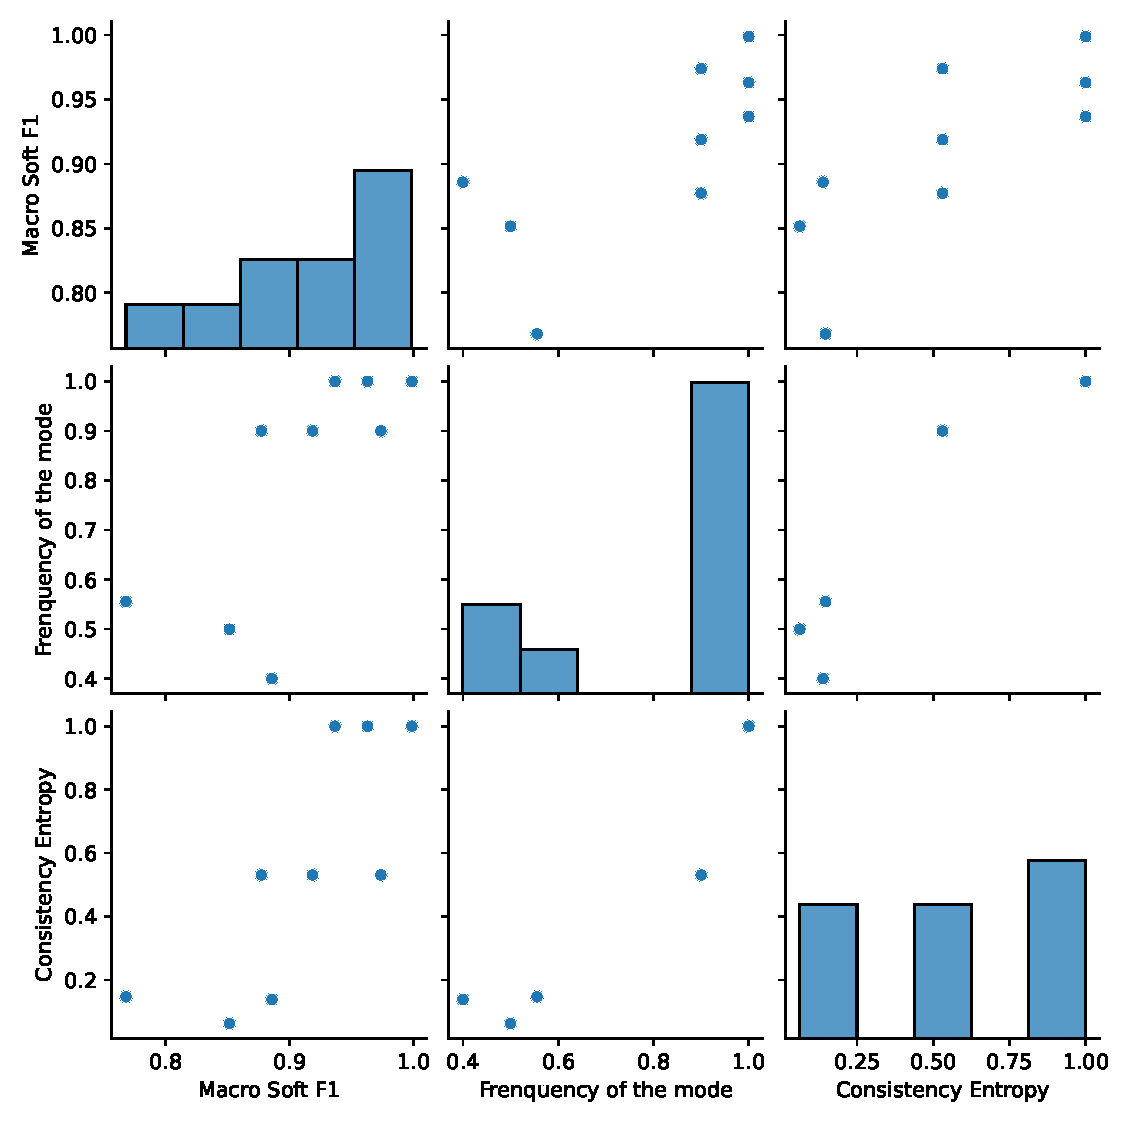
\includegraphics[width=\textwidth]{metrics_scattermatrix}
\caption{Scatter matrix of evaluation metrics. Each point represents a question.}
\label{fig:metrics_scattermatrix}
\end{figure}

The scatter matrix in Figure \ref{fig:metrics_scattermatrix} provides a clear visualization of the relationships among the performance metrics, including macro Soft F1-score, frequency of the mode, and consistency entropy. These metrics are positively correlated, indicating that better performance in one area is often associated with better performance in the others. For instance, the macro Soft F1-score correlates strongly with the frequency of the mode, suggesting that when the system achieves a good balance between precision and recall, it also produces more consistent outputs. Similarly, the macro Soft F1-score correlates with consistency entropy, meaning that higher accuracy is associated with more predictable outputs. The frequency of the mode also correlates with consistency entropy, reinforcing the observation that a higher proportion of consistent outputs is linked to greater predictability.

In Figure \ref{fig:metrics_scattermatrix}, these relationships are reflected in the positioning of data points. Questions with high performance metrics are concentrated in the upper-right corner of the graph, showing strong alignment between accuracy, consistency, and predictability. These include Q2, Q5, Q8, and Q9, which achieved high macro Soft F1-scores and consistency metrics.

In contrast, questions with lower performance metrics are scattered in the lower-left region of the graph, reflecting reduced consistency and accuracy. Examples include Q1, Q7, and Q10, which had lower macro Soft F1-scores and consistency metrics, indicating areas where the system struggled to generate accurate and consistent SQL queries.

\section{Detailed Examination of Questions}

The performance of the system can be further understood by analyzing the characteristics of both high-performing and low-performing questions. These two groups show distinct differences in terms of language clarity, SQL complexity, and data mapping requirements, which significantly influenced the system's ability to generate accurate and consistent outputs.

\subsection{High-Performing Questions}

High-performing questions, such as Q2, Q5, Q8, and Q9, demonstrated strong performance across all evaluated metrics. These questions achieved a 100\% completion rate, high macro precision and recall scores, and perfect or near-perfect macro Soft F1-scores. Additionally, they exhibited high frequency of the mode and consistency entropy values, indicating that the system consistently generated similar SQL queries for these prompts.

Several factors contributed to the strong performance of these questions. Firstly, the prompts were phrased clearly and unambiguously, reducing the likelihood of misinterpretation. For instance, Q2 (“How does the absolute distribution of one- or two-floor buildings vary across Municipios?”) explicitly specifies the variable of interest and the geographical aggregation level. Secondly, the required SQL queries for these questions involved standard aggregation functions and joins that are commonly encountered, such as \texttt{SUM} and \texttt{GROUP BY} clauses. This simplicity facilitated the system's ability to map the natural language to SQL syntax accurately. Lastly, the attributes mentioned in the questions corresponded directly to column names in the database, minimizing the need for complex transformations or reasoning. For example, in Q8, terms like “parking-accessible residential accommodations” directly map to database columns such as \lstinline!N_RHABITUAL_COM_ESTACIONAMENTO!.

%These factors collectively enabled the system to generate accurate and consistent SQL queries for high-performing questions, reflecting its proficiency in handling straightforward natural language prompts.

\subsection{Low-Performing Questions}

In contrast, low-performing questions such as Q1, Q7, and Q10 exhibited lower scores in macro Soft F1-score, frequency of the mode, and consistency entropy. Q10, in particular, had the lowest macro Soft F1-score of 0.7680 and a completion rate of 90\%, indicating that the system sometimes failed to generate a valid SQL query for this prompt.

Several challenges contributed to the lower performance of these questions. The prompts contained complex phrasing or multiple clauses, increasing the difficulty for the system to parse and interpret them correctly. For example, Q1 (“Which Freguesias have the highest percentage of buildings constructed before 1945?”) requires calculating a percentage based on multiple columns, which adds complexity. Additionally, some questions implied certain computations or data manipulations that were not explicitly stated. In Q7 (“Which Freguesias have the highest male-to-female ratio in the population?”), the system needed to recognize the requirement to handle potential division by zero, as some Freguesias might have zero females, necessitating the use of \texttt{NULLIF} in the SQL query.

Furthermore, low-performing questions often required the use of advanced SQL functions or error handling mechanisms that the system was less adept at generating. In Q10, the calculation of the unemployment rate involves adding two columns and dividing by another, with a potential division by zero, which complicates the query. The attributes mentioned in the questions did not always have a direct one-to-one mapping with database columns, requiring the system to infer or transform terms. This increased the likelihood of errors in the generated SQL.

%These challenges highlight areas where the system's natural language understanding and SQL generation capabilities could be improved, particularly in handling complex queries and ambiguous language.

\section{Visual Analysis of Generated Maps}

To further evaluate the system's performance, Figures \ref{fig:comparison_q7} and \ref{fig:comparison_q10} presents the generated maps for the two lowest-performing questions based on the macro Soft F1-score: Q7 and Q10. Visual inspection of these maps provides additional insights into the system's capabilities and limitations.

\begin{figure}[htbp]
    \centering

    % Question 7
    \begin{minipage}[b]{\textwidth}
      \centering
      \subbottom[Ground Truth\label{fig:q7_gt}]{%
        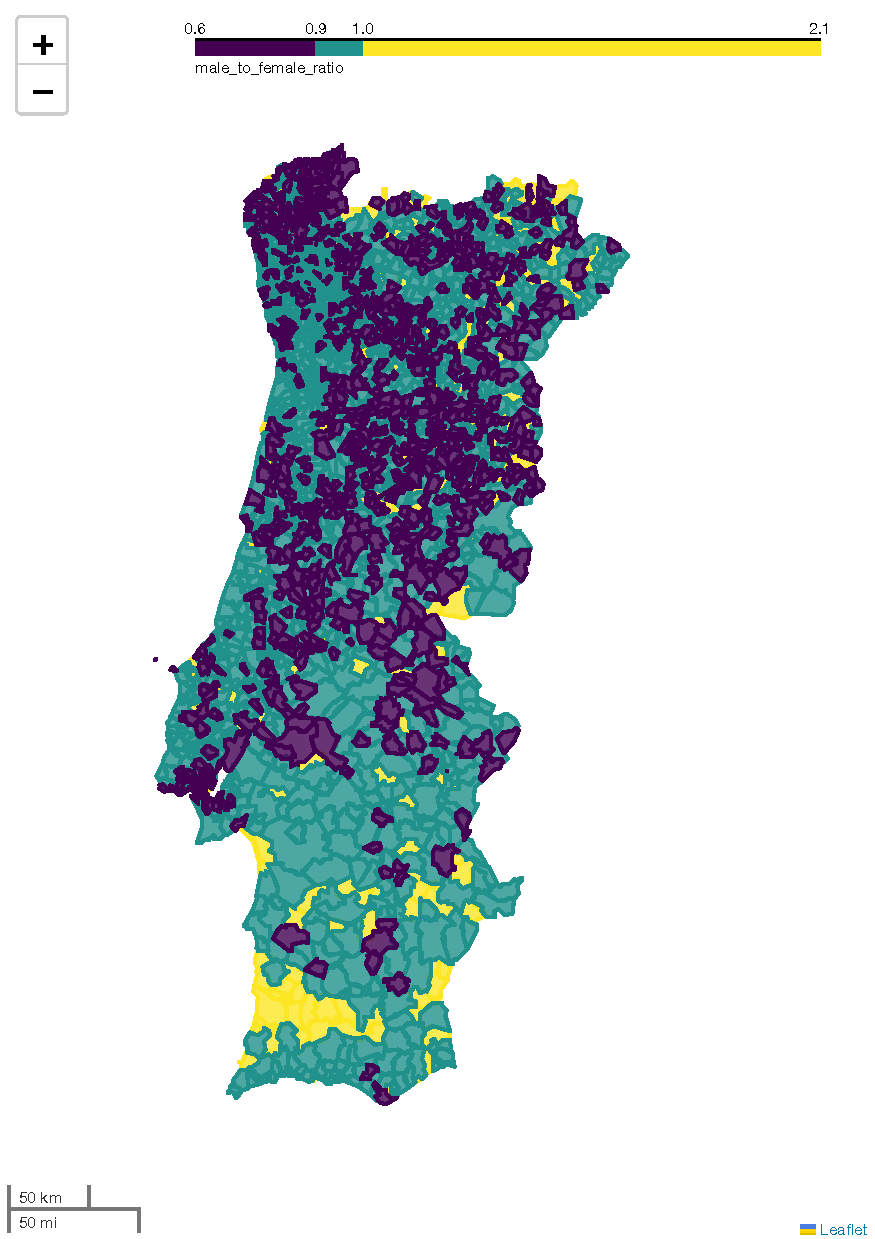
\includegraphics[width=0.5\linewidth]{q7_gt_map.html.pdf}}%
      \hfill
      \subbottom[Generated Map 1\label{fig:q7_pred1}]{%
        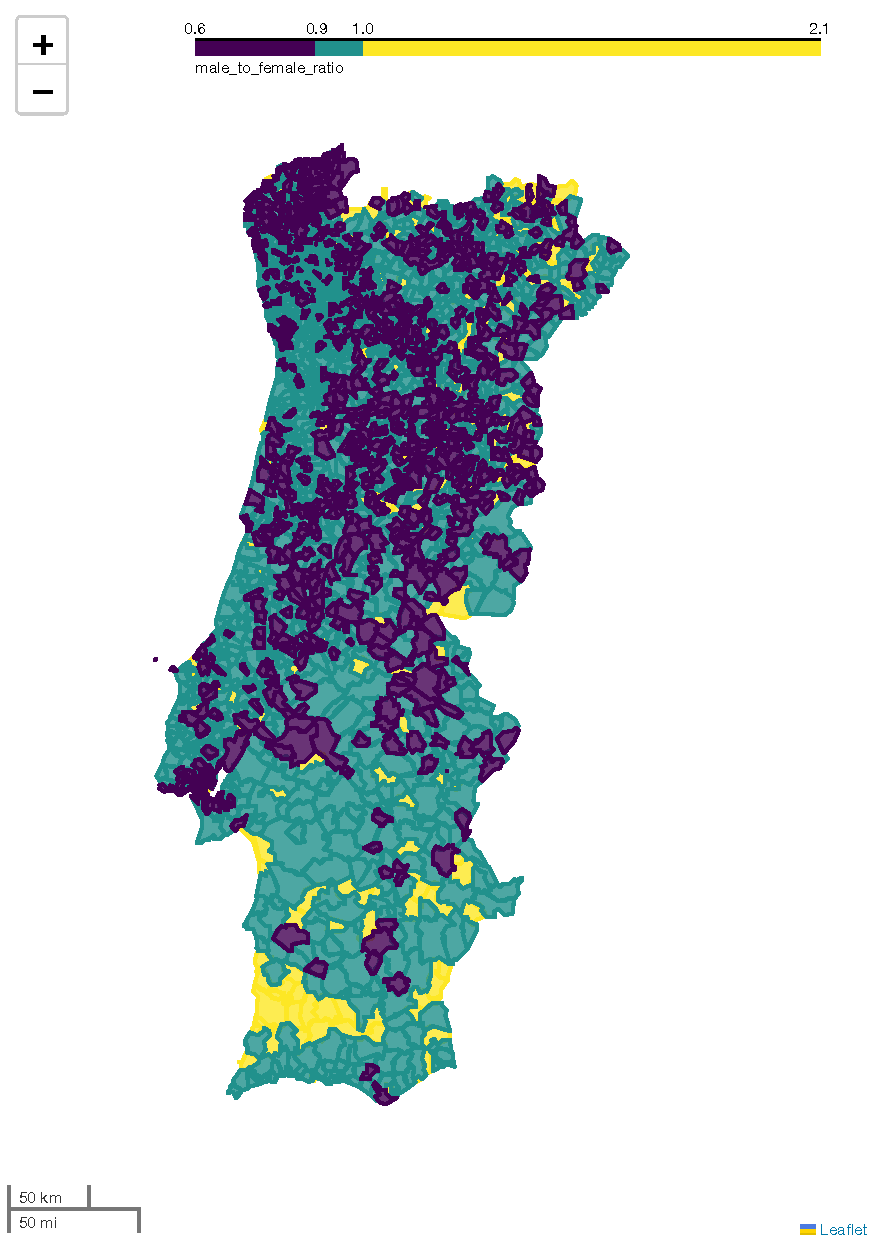
\includegraphics[width=0.5\linewidth]{q7_pred_map_1.html.pdf}}%
      \hfill
      \subbottom[Generated Map 2\label{fig:q7_pred3}]{%
        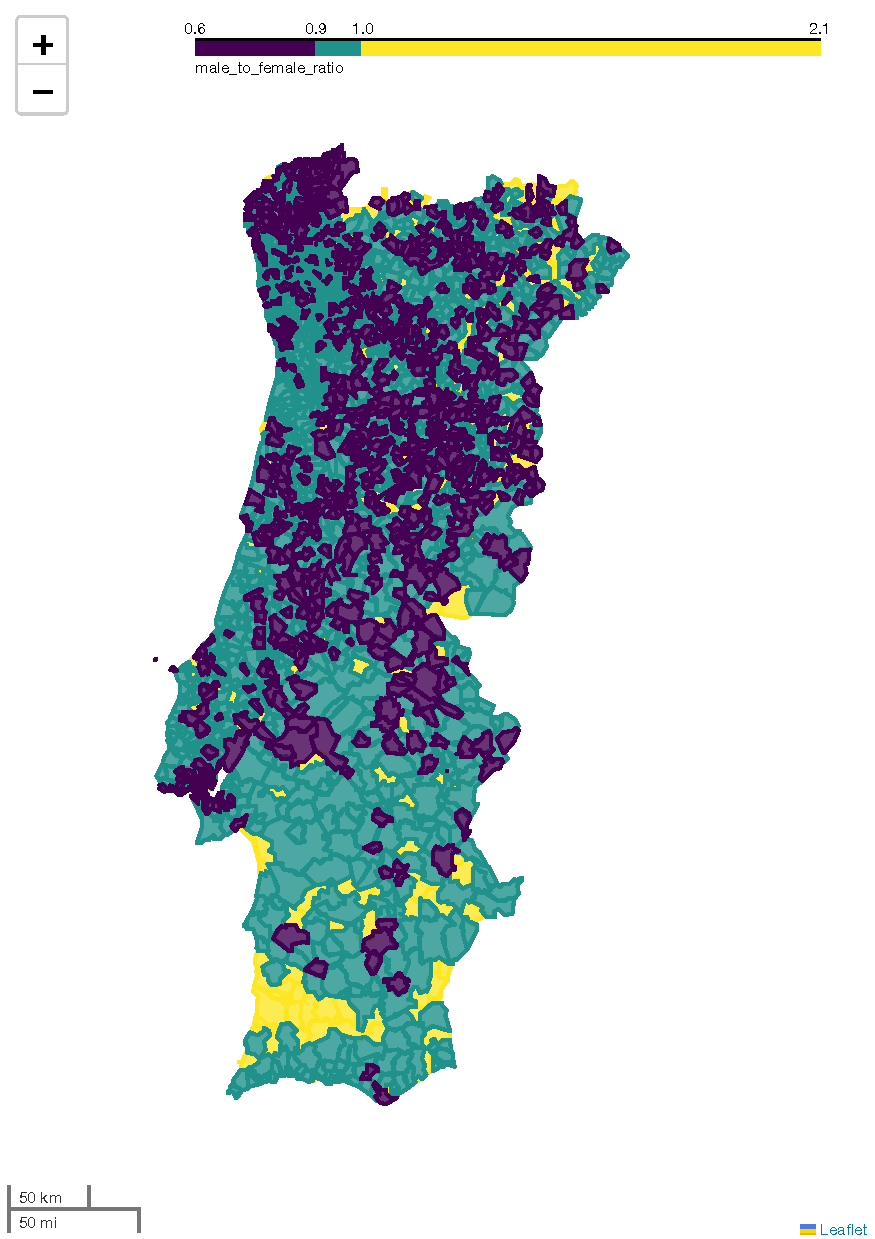
\includegraphics[width=0.5\linewidth]{q7_pred_map_3.html.pdf}}%
    \end{minipage}
    \caption{Comparison of ground truth and generated maps by Prompt2Map for Question 7: Which Freguesias have the highest male-to-female ratio in the population?}
    \label{fig:comparison_q7}
  \end{figure}



  \begin{figure}[htbp]
    \centering
    \begin{minipage}[b]{\textwidth}
      \centering
      \subbottom[Ground Truth\label{fig:q10_gt}]{%
        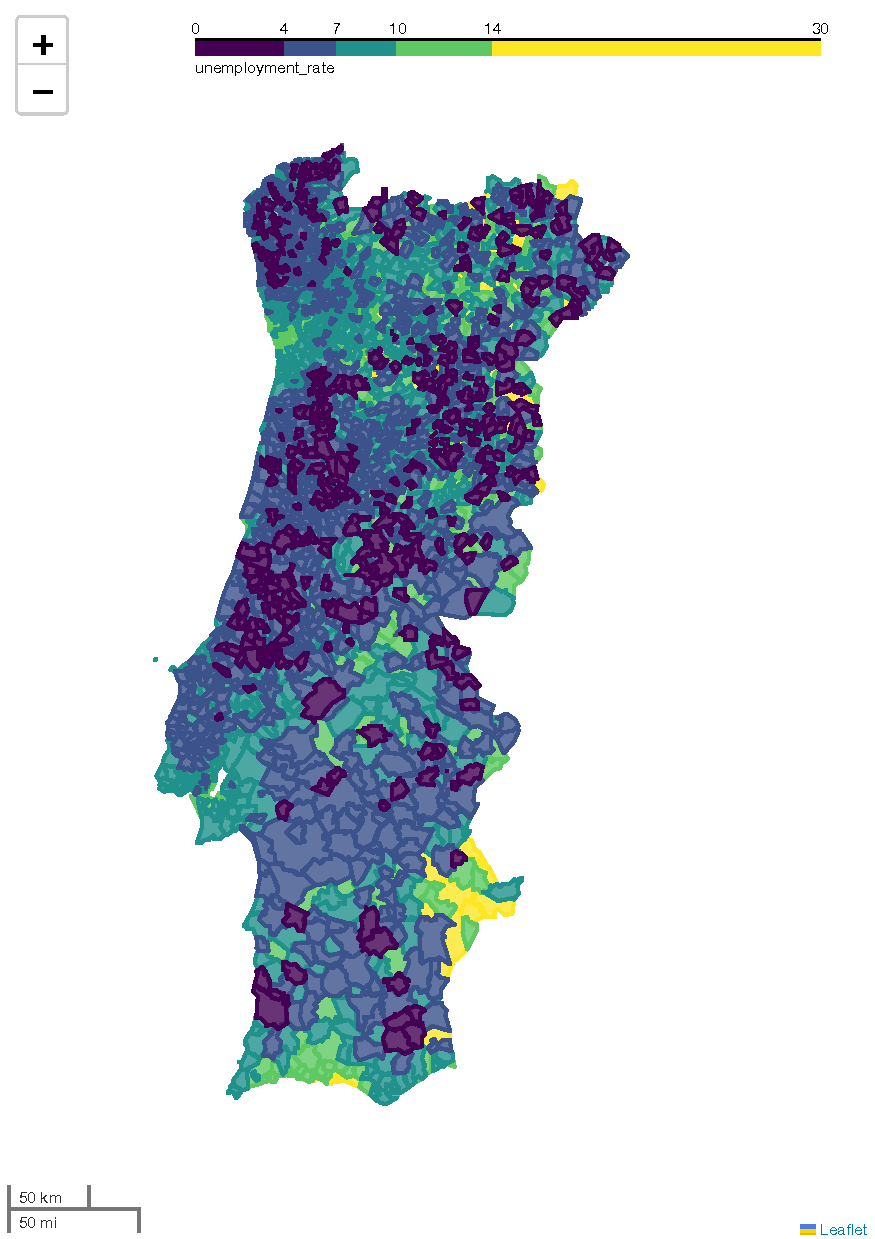
\includegraphics[width=0.5\linewidth]{q10_gt_map.html.pdf}}%
      \hfill
      \subbottom[Generated Map 1\label{fig:q10_pred1}]{%
        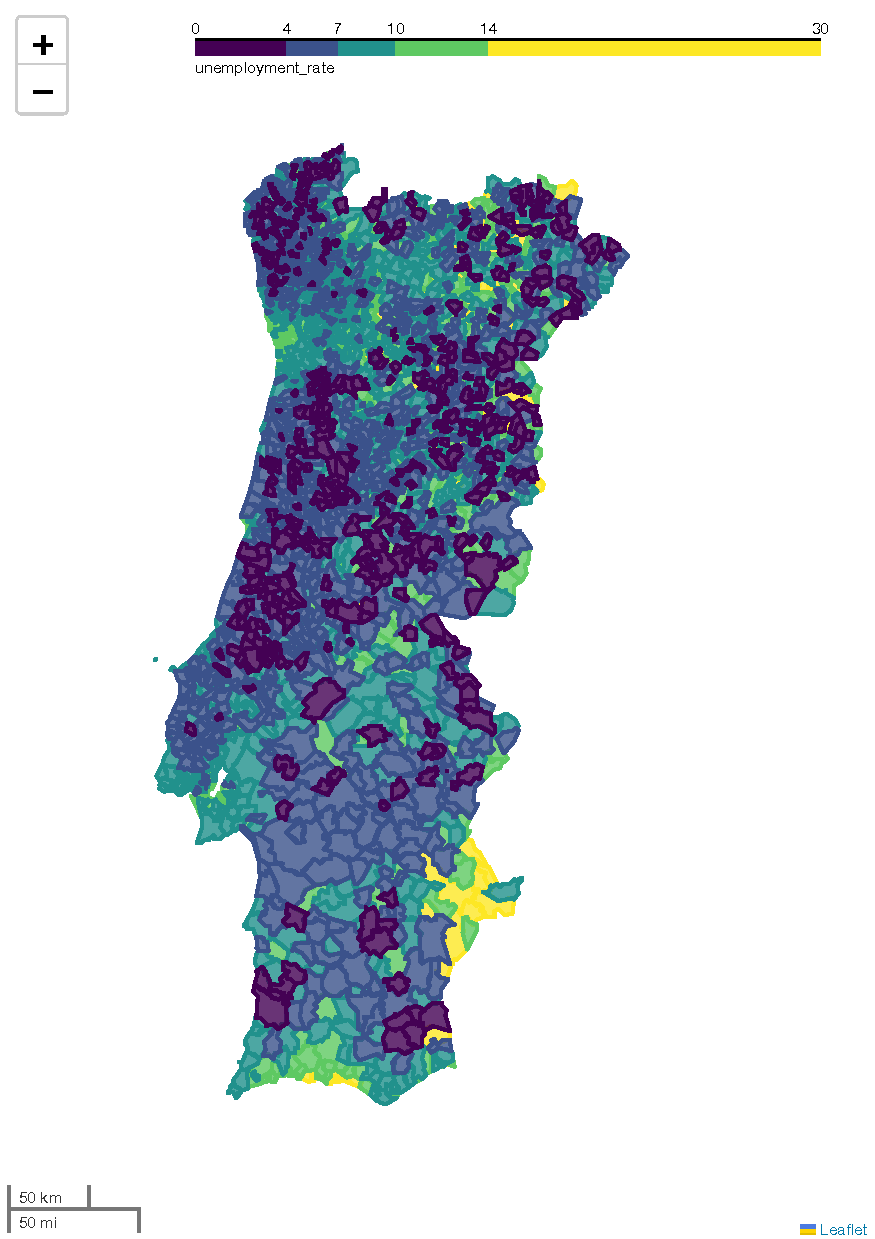
\includegraphics[width=0.5\linewidth]{q10_pred_map_1.html.pdf}}%
      \hfill
      \subbottom[Generated Map 2\label{fig:q10_pred3}]{%
        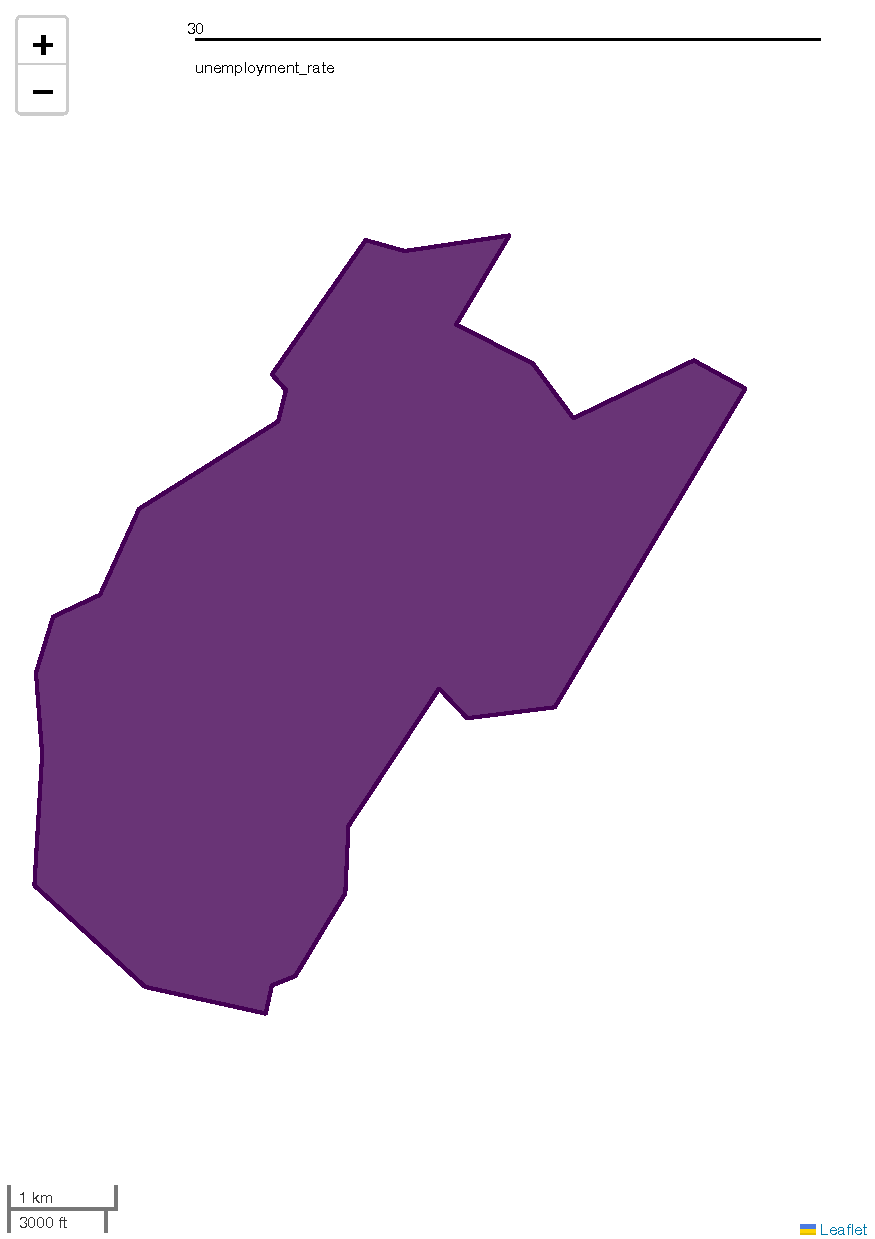
\includegraphics[width=0.5\linewidth]{q10_pred_map_3.html.pdf}}%
    \end{minipage}
    \caption{Comparison of ground truth and generated maps by Prompt2Map for Question 10: In which Freguesias is the unemployment rate highest?}
    \label{fig:comparison_q10}
  \end{figure}



\subsection{Analysis of Q7 Map}

For Q7, both generated maps are identical to the ground truth map, despite the low macro Soft F1-score. In this case, the recall is very high, indicating that the generated query is retrieving more data that it needs at the cost of losing precision. The ground truth is a subset of the generated datasets, but the extra columns are penalized, leading to a lower precision score. This discrepancy highlights a limitation of the macro Soft F1-score metric, as it penalizes the model for false positives (extra columns) even when the generated maps accurately reflect the ground truth. The high recall suggests that the system is capable of capturing all relevant data points, but the metric's sensitivity to precision results in a lower overall score. 

\subsection{Analysis of Q10 Map}

For Q10, Generated Map 1 might seem identical to the ground truth map at first glance, but it actually contains fewer rows. This discrepancy arises because the underlying SQL query is incorrect. The query groups the data by Freguesia name alone, but there are multiple Freguesias with the same name across different Municipios. Therefore, the correct approach would be to group by both Freguesia and Municipio to ensure accurate aggregation. On the other hand, Generated Map 2 displays a single feature, which we could assume represents the Freguesia with the highest unemployment rate. This result could also answer the original question, indicating potential ambiguity in the prompt that leads to inconsistent outputs. The system's interpretation of the question might vary, causing it to generate different results based on its understanding of the query requirements.


\section{Web Application}

The Prompt2Map system includes a user-friendly web application built using Streamlit\footnote{\url{https://streamlit.io}}, named Census Map GPT. This application allows users to generate maps based on census data through natural language prompts. The frontend captures the user's intent and translates it into SQL queries, which are then used to retrieve and visualize the relevant data.

Figure~\ref{fig:prompt2map_ui} illustrates the interface of the Census Map GPT application. Subfigure~\ref{fig:subfig1} shows the prompt input area where users can type their queries. Subfigure~\ref{fig:subfig2} displays the generated map based on the user's prompt. Subfigure~\ref{fig:subfig3} presents the data retrieved from the database, and subfigure~\ref{fig:subfig4} shows the SQL query generated from the user's prompt.

\begin{figure}[htbp]
  \centering
  \subbottom[Prompt to generate a map\label{fig:subfig1}]{%
    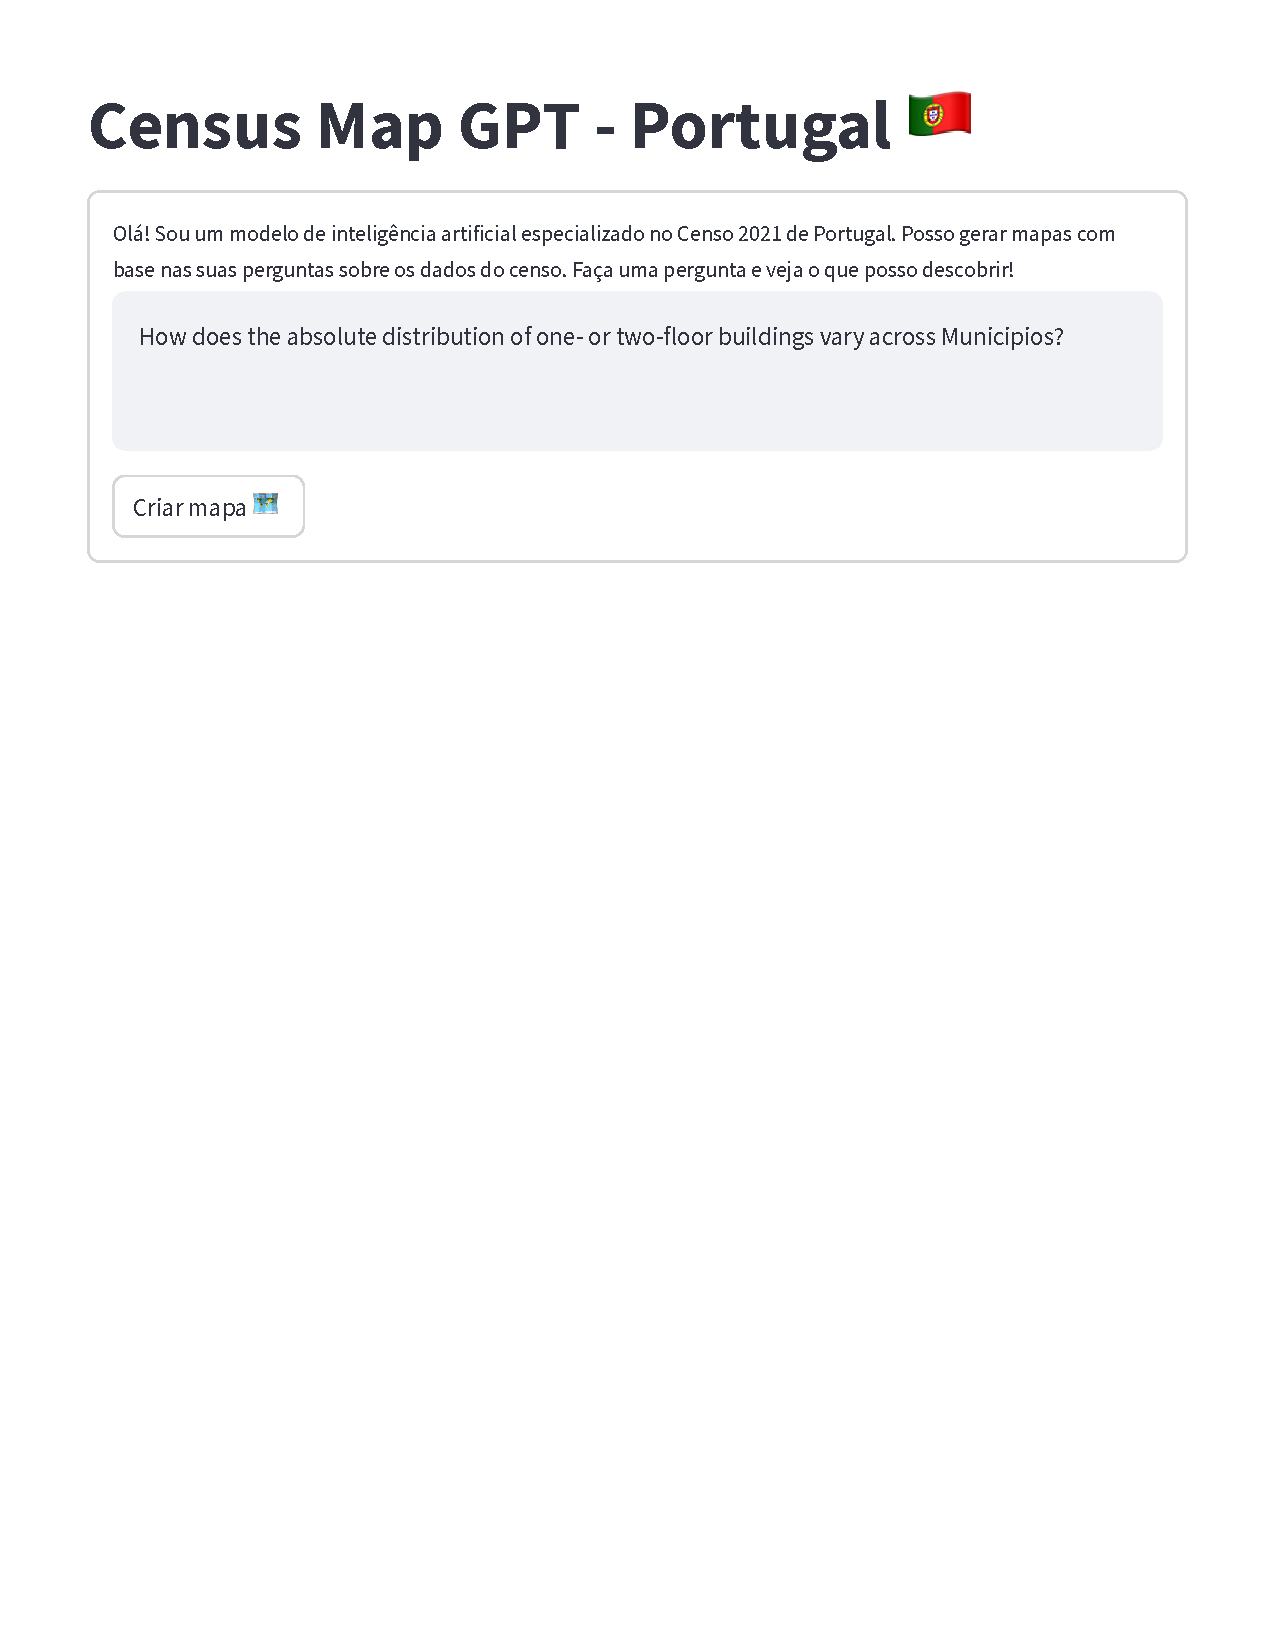
\includegraphics[width=0.5\linewidth]{censusmapgpt_1}}%
  \subbottom[Generated map\label{fig:subfig2}]{%
    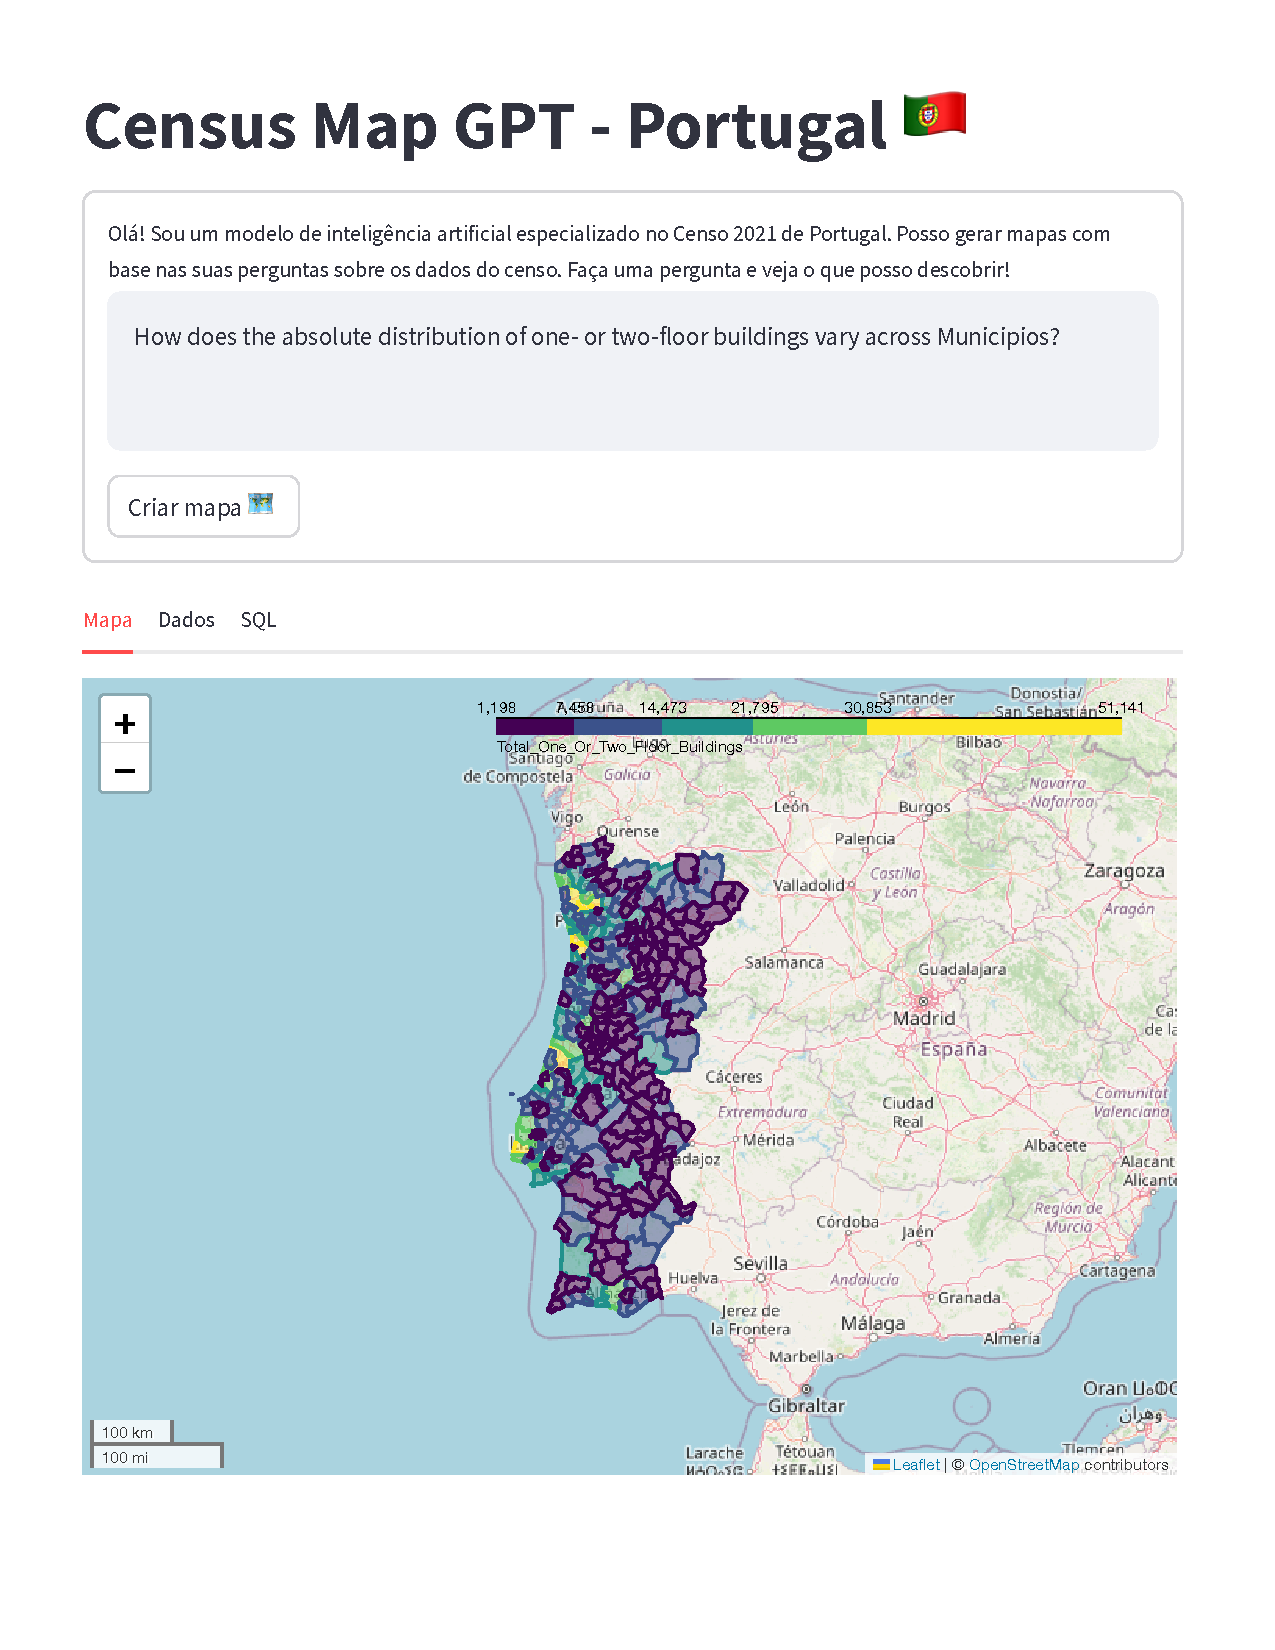
\includegraphics[width=0.5\linewidth]{censusmapgpt_2}}\\
  \subbottom[Generated data\label{fig:subfig3}]{%
    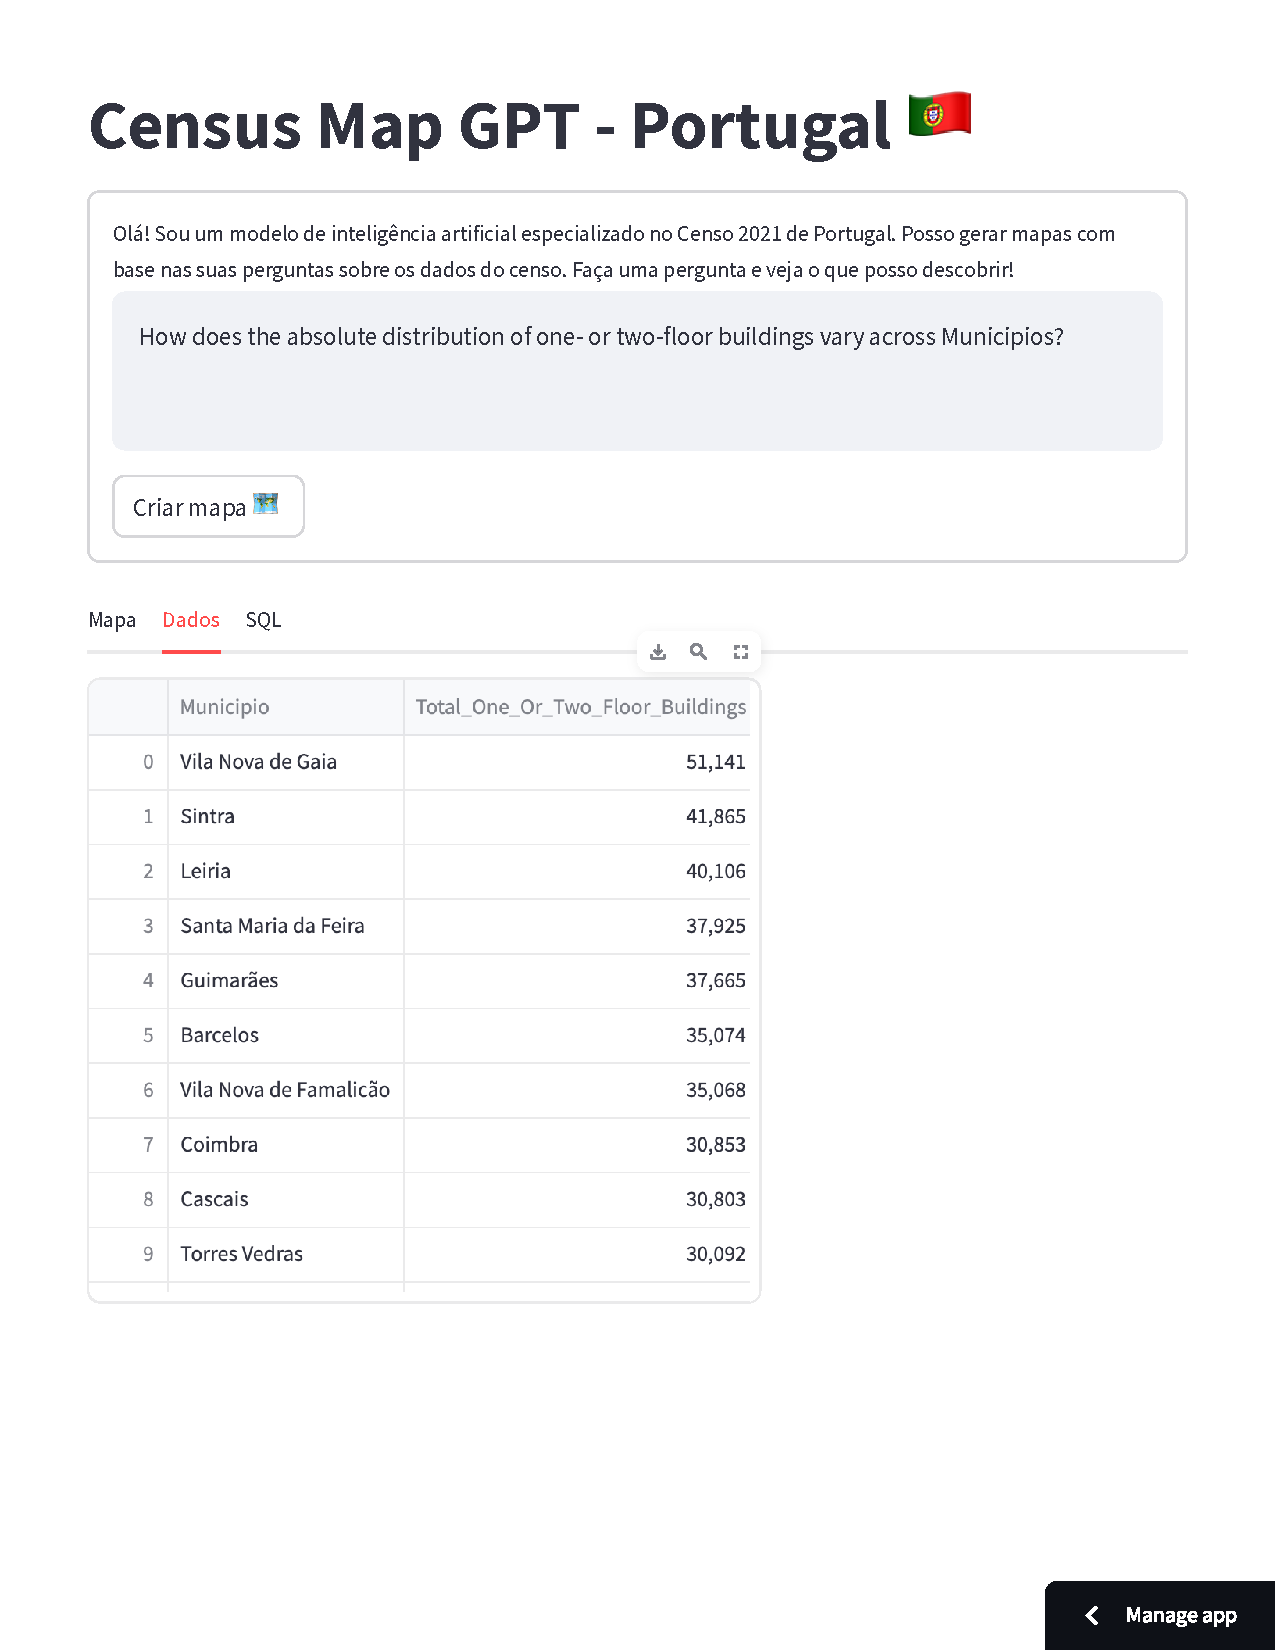
\includegraphics[width=0.5\linewidth]{censusmapgpt_3}}%
  \subbottom[Generated SQL\label{fig:subfig4}]{%
    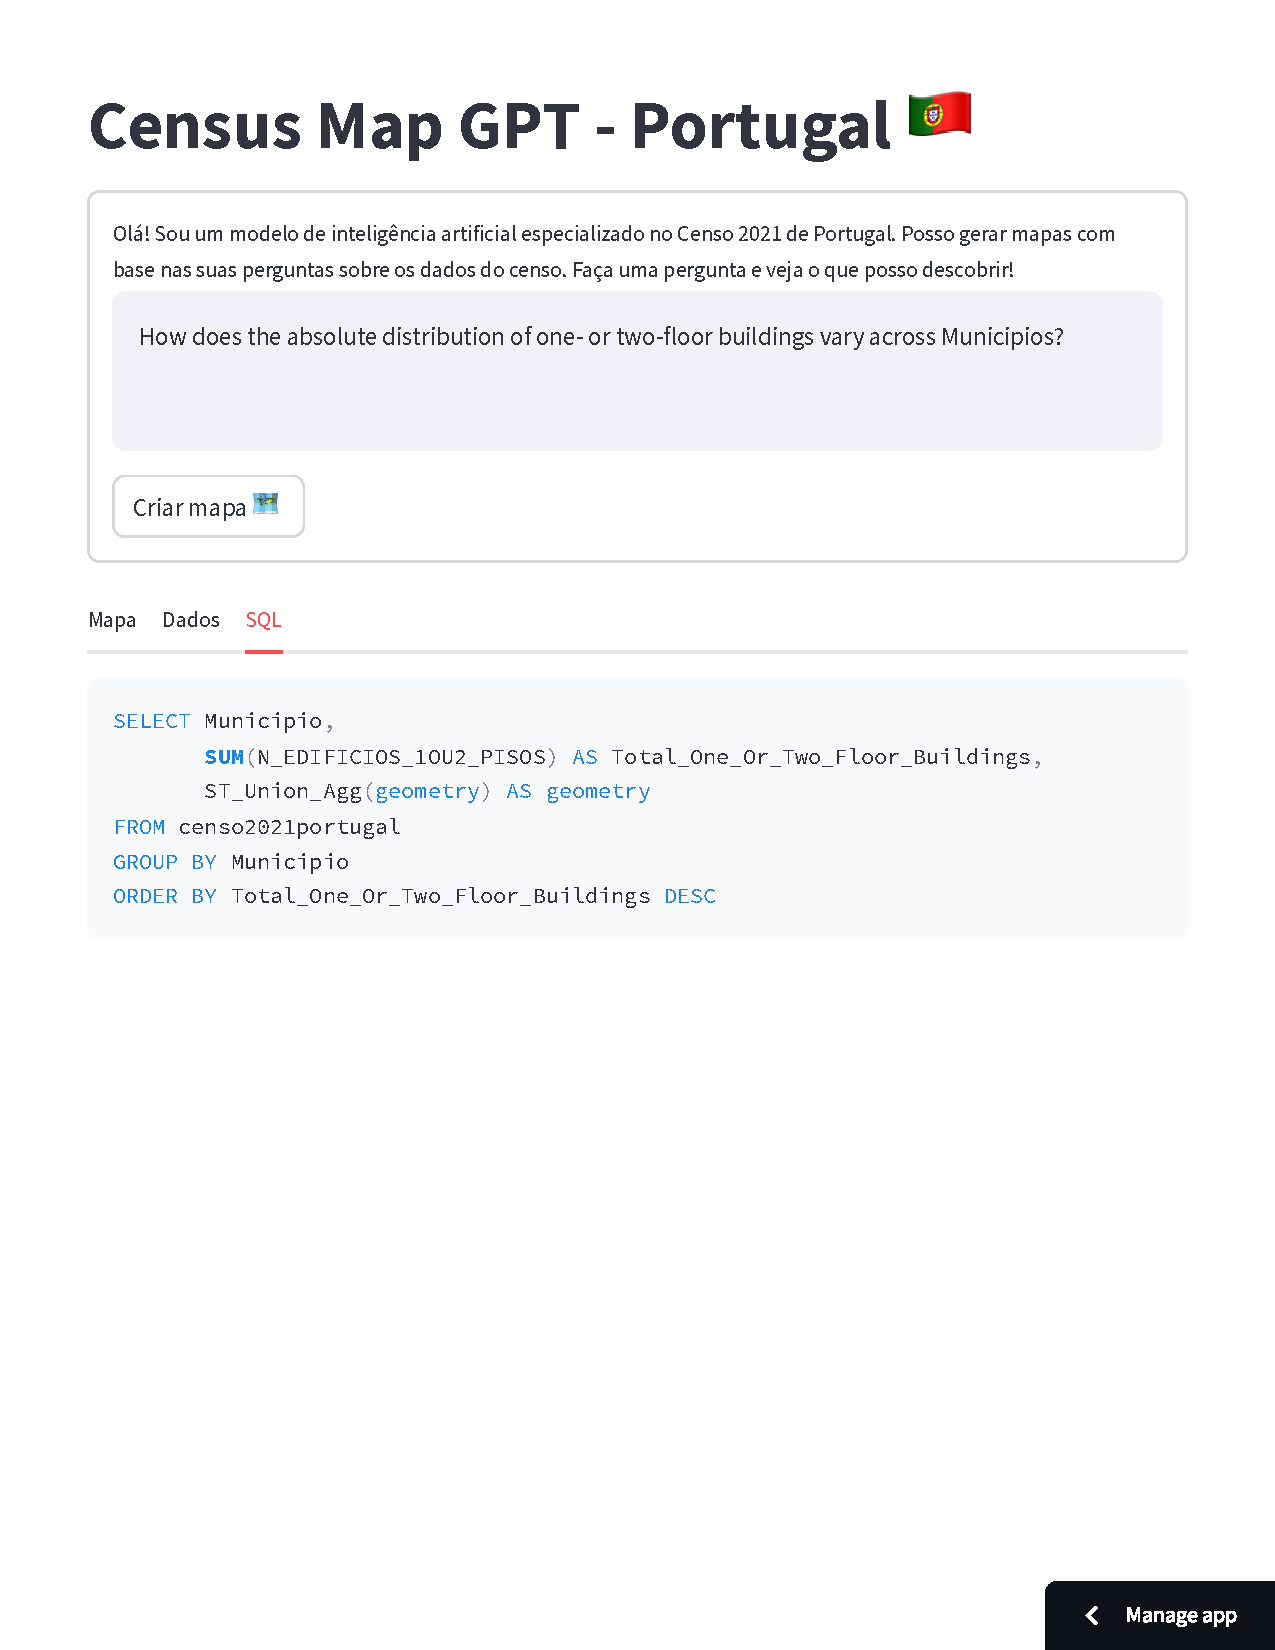
\includegraphics[width=0.5\linewidth]{censusmapgpt_4}}%
  \caption{Census Map GPT UI for Prompt2Map}
  \label{fig:prompt2map_ui}
\end{figure}

The web application enhances accessibility by allowing users without technical expertise in SQL or data visualization tools to interact with complex datasets effectively. By leveraging natural language processing, the system simplifies the process of data retrieval and visualization, making it more intuitive and efficient.